\documentclass[11pt, a4paper, oneside,final,notitlepage,onecolumn]{article}\usepackage[]{graphicx}\usepackage[]{color}
%% maxwidth is the original width if it is less than linewidth
%% otherwise use linewidth (to make sure the graphics do not exceed the margin)
\makeatletter
\def\maxwidth{ %
  \ifdim\Gin@nat@width>\linewidth
    \linewidth
  \else
    \Gin@nat@width
  \fi
}
\makeatother

\definecolor{fgcolor}{rgb}{0.345, 0.345, 0.345}
\newcommand{\hlnum}[1]{\textcolor[rgb]{0.686,0.059,0.569}{#1}}%
\newcommand{\hlstr}[1]{\textcolor[rgb]{0.192,0.494,0.8}{#1}}%
\newcommand{\hlcom}[1]{\textcolor[rgb]{0.678,0.584,0.686}{\textit{#1}}}%
\newcommand{\hlopt}[1]{\textcolor[rgb]{0,0,0}{#1}}%
\newcommand{\hlstd}[1]{\textcolor[rgb]{0.345,0.345,0.345}{#1}}%
\newcommand{\hlkwa}[1]{\textcolor[rgb]{0.161,0.373,0.58}{\textbf{#1}}}%
\newcommand{\hlkwb}[1]{\textcolor[rgb]{0.69,0.353,0.396}{#1}}%
\newcommand{\hlkwc}[1]{\textcolor[rgb]{0.333,0.667,0.333}{#1}}%
\newcommand{\hlkwd}[1]{\textcolor[rgb]{0.737,0.353,0.396}{\textbf{#1}}}%

\usepackage{framed}
\makeatletter
\newenvironment{kframe}{%
 \def\at@end@of@kframe{}%
 \ifinner\ifhmode%
  \def\at@end@of@kframe{\end{minipage}}%
  \begin{minipage}{\columnwidth}%
 \fi\fi%
 \def\FrameCommand##1{\hskip\@totalleftmargin \hskip-\fboxsep
 \colorbox{shadecolor}{##1}\hskip-\fboxsep
     % There is no \\@totalrightmargin, so:
     \hskip-\linewidth \hskip-\@totalleftmargin \hskip\columnwidth}%
 \MakeFramed {\advance\hsize-\width
   \@totalleftmargin\z@ \linewidth\hsize
   \@setminipage}}%
 {\par\unskip\endMakeFramed%
 \at@end@of@kframe}
\makeatother

\definecolor{shadecolor}{rgb}{.97, .97, .97}
\definecolor{messagecolor}{rgb}{0, 0, 0}
\definecolor{warningcolor}{rgb}{1, 0, 1}
\definecolor{errorcolor}{rgb}{1, 0, 0}
\newenvironment{knitrout}{}{} % an empty environment to be redefined in TeX

\usepackage{alltt}%
\usepackage{amsmath}
\usepackage{amssymb}
% \usepackage{sw20lart}%
% @@take out the above!?
\setcounter{MaxMatrixCols}{30}%
\usepackage{amsfonts}%
\usepackage{graphicx}
% TCIDATA{OutputFilter=latex2.dll}
% TCIDATA{Version=5.00.0.2570}
% TCIDATA{TCIstyle=Article/art4.lat,lart,article}
% TCIDATA{LastRevised=Tuesday, October 12, 2010 11:16:48}
% TCIDATA{<META NAME="GraphicsSave" CONTENT="32">}
% TCIDATA{<META NAME="SaveForMode" CONTENT="3">}
% TCIDATA{Language=American English}
\setlength{\oddsidemargin}{-0.00in}
\setlength{\textwidth}{6.2in}
\setlength{\topmargin}{-0.75in}
\setlength{\textheight}{9.7in}
\newtheorem{THEOREM}{\rm THEOREM}
\newtheorem{DEFINITIO}[THEOREM]{\rm
  DEFINITION}
\newenvironment{DEFINITION}{\begin{DEFINITIO}
    \rm}{\end{DEFINITIO}}
\newtheorem{LEMMA}[THEOREM]{\rm LEMMA}
\newtheorem{LEMMAX}[THEOREM]{\hspace{1 em}\rm LEMMA}
\newtheorem{COROLLARY}[THEOREM]{\rm
  COROLLARY}
\newtheorem{COROLLARYX}[THEOREM]{\hspace{1 em}\rm
  COROLLARY}
\newtheorem{ASSUMPTIO}[THEOREM]{\rm
  ASSUMPTION}
\newenvironment{ASSUMPTION}{\begin{ASSUMPTIO}
    \rm}{\end{ASSUMPTIO}}
\newtheorem{REMAR}[THEOREM]{\rm REMARK}
\newenvironment{REMARK}{\begin{REMAR}
    \rm}{\end{REMAR}}
\newtheorem{CLAI}[THEOREM]{\rm
  CLAIM}
\newenvironment{CLAIM}{\begin{CLAI}
    \rm}{\end{CLAI}}
\newtheorem{CONCLUSION}[THEOREM]{\rm
  CONCLUSION}
\newtheorem{OBSERVATION}[THEOREM]{\rm
  OBSERVATION}
\newtheorem{PROPOSITION}[THEOREM]{\rm
  PROPOSITION}
\newtheorem{EXAMPL}[THEOREM]{\rm EXAMPLE}
\newenvironment{EXAMPLE}{\begin{EXAMPL}
    \rm}{\end{EXAMPL}}
\newcounter{AA}
\newcounter{subsectio}
\newcounter{sectio}
\def\xt{\par\hangafter=
  1\hangindent=\parindent\noindent}
\renewcommand{\baselinestretch}{2}
\newcommand{\ga}{\alpha}
\newcommand{\xb}{\beta}
\newcommand{\xg}{\gamma}
\newcommand{\gd}{\delta}
\newcommand{\gdd}{\Delta}
\newcommand{\xe}{\epsilon}
\newcommand{\gf}{\varphi}
\newcommand{\gk}{\kappa}
\newcommand{\gl}{\lambda}
\newcommand{\gm}{\mu}
\newcommand{\gn}{\nu}
\newcommand{\gp}{\pi}
\newcommand{\gpp}{\Pi}
\newcommand{\gr}{\rho}
\newcommand{\gs}{\sigma}
\newcommand{\gss}{\Sigma}
\newcommand{\gt}{\tau}
\newcommand{\gw}{\omega}
\newcommand{\gww}{\Omega}
\newcommand{\Naoud}{I\hspace{-0.193em}N}
\newcommand{\Roud}{I\hspace{-0.26em}R}
\newcommand{\Na}{I\kern -3pt N}
\newcommand{\R}{\mathbb{R}}
\newcommand{\cir}{\!\circ\!}
\newcommand{\bd}{$\bullet$}
\newcommand{\elt}{\!\in\!}
\newcommand{\ggeq}{\geqslant}
\newcommand{\ve}{\!\vee\!}
\newcommand{\wedg}{\!\wedge\!}
\newcommand{\E}{\exists}
\newcommand{\ep}{~\hfill $\square$}
\newcommand{\ey}{\emptyset}
\newcommand{\FA}{\forall}
\newcommand{\iy}{\infty}
\newcommand{\La}{\Leftarrow}
\newcommand{\Lra}{\Leftrightarrow}
\newcommand{\lleq}{\leqslant}
\newcommand{\mo}{\mapsto}
\newcommand{\noi}{\noindent}
\newcommand{\p}{\succcurlyeq}
\newcommand{\rp}{\preccurlyeq}
\newcommand{\srp}{\prec}
\newcommand{\ra}{\rightarrow}
\newcommand{\Ra}{\Rightarrow}
\newcommand{\sbs}{\subset}
\newcommand{\sps}{\supset}
\newcommand{\SA}{{\cal A}}
\newcommand{\SB}{{\cal B}}
\newcommand{\SC}{{\cal C}}
\newcommand{\SD}{{\cal D}}
\newcommand{\SF}{{\cal F}}
\newcommand{\SP}{{\cal P}}
\newcommand{\SQ}{{\cal Q}}
\newcommand{\ST}{{\cal T}}
\newcommand{\SU}{{\cal U}}
% BeginMSIPreambleData
\ifx\pdfoutput\relax\let\pdfoutput=\undefined\fi
\newcount\msipdfoutput
\ifx\pdfoutput\undefined\else
\ifcase\pdfoutput\else
\msipdfoutput=1
\ifx\paperwidth\undefined\else
\ifdim\paperheight=0pt\relax\else\pdfpageheight\paperheight\fi
\ifdim\paperwidth=0pt\relax\else\pdfpagewidth\paperwidth\fi
\fi\fi\fi
% EndMSIPreambleData

% % \usepackage{changepage}
% \usepackage{rotating}
\renewcommand{\tabcolsep}{3pt}

\usepackage{longtable}
%% \usepackage{rotating} 
%% \renewenvironment{table*}[1][1]{
%%   % \setlength{\columnsep}{1pt}  
%%   % \renewcommand{\tabcolsep}{2pt}
%% \begin{table}[#1]\footnotesize
%%   \begin{adjustwidth}{-0.2cm}{}
%%   }{
%%   \end{adjustwidth}
%% \end{table}}

\renewcommand{\thetable}{WA\arabic{table}}
\renewcommand{\thefigure}{WA\arabic{figure}}
\IfFileExists{upquote.sty}{\usepackage{upquote}}{}
\begin{document}

\title{\vspace{-1\baselineskip}\textbf{Web Appendix to:\\
 An Experimental Test of Prospect Theory for Predicting Choice under Ambiguity\vspace{0\baselineskip}}}
\author{Amit Kothiyal$^a$, Vitalie Spinu$^b$, \& Peter P.\ Wakker$^b$\\
  $^a$ Max Planck Institute for Human Development,
  Lentzeallee 94,\\ 14195 Berlin, Germany\\
  $^b$ Econometric Institute, Erasmus University,
  \\P.O.\ Box 1738, Rotterdam, 3000 DR, the Netherlands\\~}

 \date{\vspace{0\baselineskip}December, 2012}
\maketitle

We discuss the fitting procedure in more detail, and report the median values of individual parameters that we estimated for various models. For source prospect theory (SPT) we provide all the parameter estimates for all subjects. We conclude with the model tournament table computed based on different fitting/test splits of the data (cross validation) than that of HLM.  References and notation are as in the main text.




\section{Additional remarks on the estimation method}
\label{sec:design}

As pointed out in the main text, all models were fit individual by individual, and predicted likelihoods were used to compare the models. We here follow the technique used by HLM (Hey, Lotito, \& Maffioletti 2010). Some additional remarks are due. 

The advantage of fitting the data individual by individual is mainly computational -- the number of parameters estimated are in the range of 3-10 per subject, which given the amount of choice data (135 binary responses per subject) gives a stable fit for most cases. Moreover, the maximum likelihood optimization algorithm (we used Nelder-Mead) converges fast. The disadvantage of individual fitting is two-fold.

First, individual fitting does not take into account the information about the choices and parameters of other subjects. In statistics, taking such information into account is known as a collective inference -- given the parameters or choices of a group of subjects we can infer the parameters and predict choices of other individuals. Thus it may be interesting to to pool all the data and estimate the parameters for all individuals at the same time. This procedure obviously requires additional assumptions at the population level. Mixed effect models and hierarchical Bayesian inference are two standard approaches that can be used. We estimated a mixed effect for SPT and it gave results  virtually identical to the individual by individual estimates. Because the optimization procedure is very complex (240 parameters and more than 400 inequality restrictions) and does not give an obvious gain over the individual by individual estimation we did not pursue this method further.

The second problem of individual by individual estimation is that it can lead to overfitting.  It does so for several subjects for almost all models we considered. It happens when a subject's choice data (used for fitting) is fit ``too'' well by a deterministic model and, hence, the $\sigma$ parameter (representing the model fitting error) becomes too small. As a consequence the model generalizes poorly and predicts very poorly on the test set. To address this issue, HLM removed subject 35 who gave very bad predicted log-likelihoods for multiple prior models.\footnote{Tables~\ref{table_A_mean_plike} and~\ref{table_A_winners_with_SPT} below are counterparts to Tables~1 and~2 from the main text with the subject 35 included.} An alternative way out is to use more robust measures of central tendency, such as medians or trimmed means, and to perform  non-parametric statistical tests without removing any subjects, as reported in the main text.  
 %v.k. refer to table in paper after publication.

To reduce the impact of overfitting, HLM also restricted the error parameter $\sigma$ by imposing the lower bound of $0.01$ for all models. We follow the same strategy in our estimations. This is not a serious restriction as it affects only a small number of individuals for our main model, SPT, as can be seen in Figure~\ref{fig:sigma_par_boxplot}. It is also empirically plausible to assume a minimal level of error and no perfect fit.  In general, the more parameters a model has, the more prone it is to overfitting, and the more subjects will have an estimated sigma equal to the lower bound.  We similarly imposed an additional restriction on prospect theory models
 -- we did not allow the individual loss aversion parameter $\lambda$ to exceed $40$.  Again, this is empirically plausible and it avoids degenerate estimates.

\begin{figure}
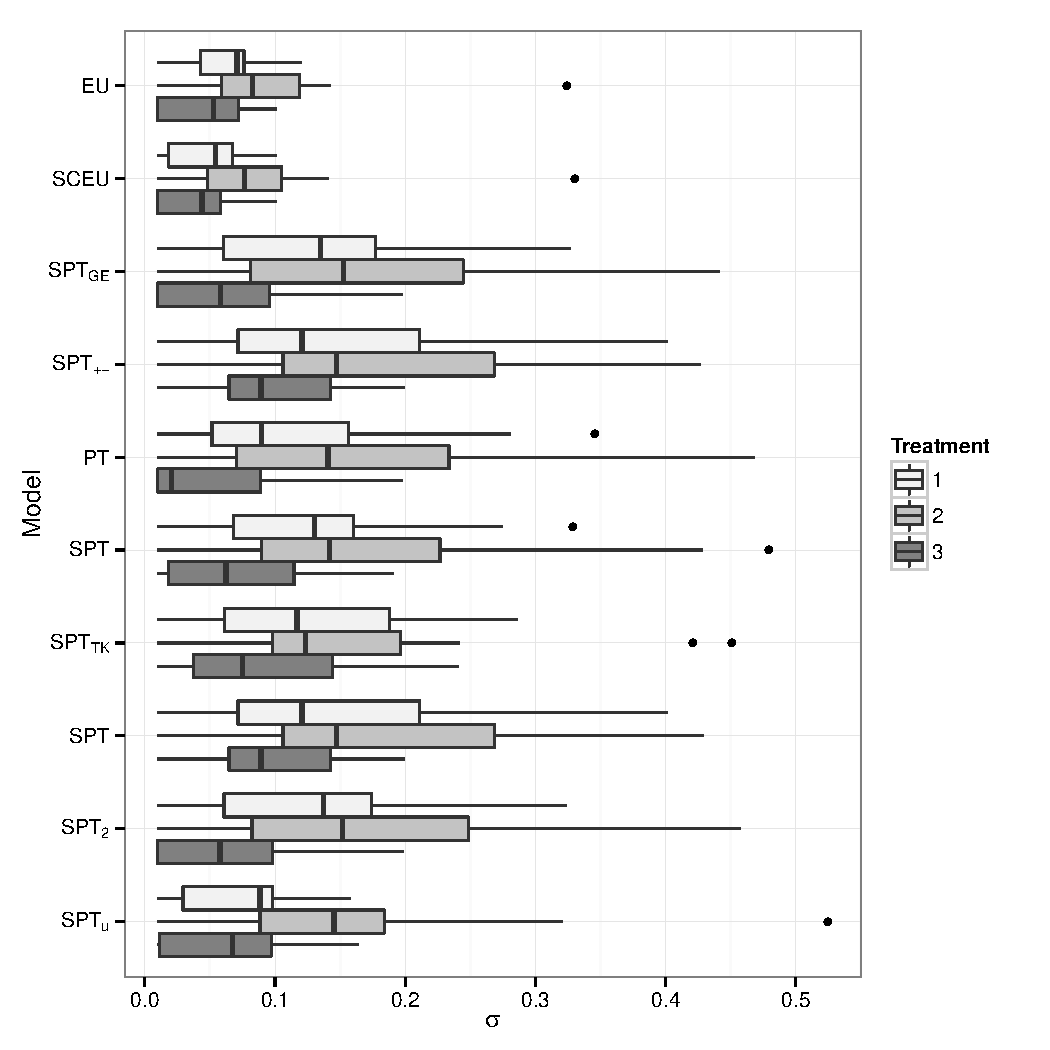
\includegraphics[width=\maxwidth]{figure/sigma_par_boxplot-1} \caption[Boxplots of estimats of the error parameter ]{Boxplots of estimats of the error parameter $\sigma$ for all variations of PT considered in the papper. The body of each box is formed by 25\%, 50\% and 75\% quantiles. The upper whisker is given by the largest observation smaller than 25\% quantile plus 1.5*IQR (inter-quantile range). Observations larger than this number are considered outliers. Lower whiskers are defined symmetrically.}\label{fig:sigma_par_boxplot}
\end{figure}




We also reproduce Tables 1 and 2 from the main text with subject 35 included.  The  MnEU and $\alpha$MM  models are seriously affected by this inclusion.

% latex table generated in R 3.1.1 by xtable 1.7-4 package
% Tue Jun 16 15:28:43 2015
\begin{table}[!htb]
\centering
\begin{tabular}{rrrrrrrrrrrr}
  \hline
 & SPT & MxEU & EU & DFT & CEU & EV & MnEU & $\alpha$MM & MaxMin & MaxMax & MinReg \\ 
  \hline
All & -3.95 & -4.02 & -4.52 & -4.70 & -6.15 & -11.49 & -12.57 & -12.58 & -13.32 & -13.97 & -14.55 \\ 
  1 & -2.60 & -2.82 & -3.44 & -3.50 & -3.22 & -12.15 & -3.13 & -2.79 & -12.57 & -14.52 & -14.48 \\ 
  2 & -5.20 & -5.14 & -5.61 & -5.93 & -6.35 & -11.03 & -5.70 & -5.58 & -14.17 & -14.45 & -14.86 \\ 
  3 & -3.90 & -3.96 & -4.39 & -4.53 & -8.68 & -11.34 & -28.73 & -29.19 & -13.14 & -12.94 & -14.29 \\ 
   \hline
\end{tabular}
\caption{Mean predicted log likelihoods for the three treatments, and overall (subject 35 included).} 
\label{table_A_mean_plike}
\end{table}
% latex table generated in R 3.1.1 by xtable 1.7-4 package
% Tue Jun 16 15:28:43 2015
\begin{table}[!htb]
\centering
\begin{tabular}{rrrrrrrrrrrr}
  \hline
 & SPT & DFT & CEU & MxEU & $\alpha$MM & EU & MnEU & EV & MaxMax & MaxMin & MinReg \\ 
  \hline
All & 9 & 8 & 7 & 7 & 6 & 5 & 4 & 1 & 1 & 0 & 0 \\ 
  1 & 2 & 3 & 3 & 4 & 1 & 0 & 2 & 0 & 0 & 0 & 0 \\ 
  2 & 4 & 2 & 3 & 1 & 2 & 4 & 0 & 1 & 0 & 0 & 0 \\ 
  3 & 3 & 3 & 1 & 2 & 3 & 1 & 2 & 0 & 1 & 0 & 0 \\ 
   \hline
\end{tabular}
\caption{Number of subject for whom a theory predicts best (subject 35 included).} 
\label{table_A_winners_with_SPT}
\end{table}


\section{Predicted likelihoods for Prospect Theory models}
\label{sec:pred-likel-prosp}

Table~\ref{table_means_PT_models}\footnote{The aggregated predicted likelihoods of $SPT$ and $SPT_{\pm}$ differ in their third decimals.  Individual predicted likelihoods are also very close.} presents medians and trimmed means of predicted likelihood for all variations of prospect theory.

% latex table generated in R 3.1.1 by xtable 1.7-4 package
% Tue Jun 16 15:28:43 2015
\begin{table}[!htb]
\centering
\begin{tabular}{rrrrr}
  \hline
 & mean$_{.1}$ & mean$_{.05}$ & mean & median \\ 
  \hline
SPT$_{\pm}$ & -3.53 & -3.62 & -3.83 & -3.32 \\ 
  SPT & -3.54 & -3.63 & -3.85 & -3.32 \\ 
  SPT$_{u}$ & -3.56 & -3.67 & -3.92 & -3.37 \\ 
  SCEU & -3.63 & -3.73 & -3.98 & -3.37 \\ 
  SPT$_{NA}$ & -3.64 & -3.91 & -6.21 & -3.13 \\ 
  SPT$_{2}$ & -3.87 & -4.06 & -4.91 & -3.03 \\ 
  SPT$_{GE}$ & -3.92 & -4.09 & -4.28 & -3.12 \\ 
  SPT$_{TK}$ & -4.19 & -4.27 & -4.39 & -4.16 \\ 
  EU & -4.34 & -4.36 & -4.43 & -4.33 \\ 
  PT & -5.10 & -5.67 & -14.42 & -3.84 \\ 
  SCEV & -11.68 & -11.61 & -11.40 & -11.60 \\ 
  SPT$_{\lambda = 1}$ & -11.74 & -11.66 & -11.45 & -12.04 \\ 
   \hline
\end{tabular}
\caption{Means, trimmed means and medians for all PT models (sorted on trimmed mean$_{.1})$.} 
\label{table_means_PT_models}
\end{table}



\section{Parameter estimates}
\label{sec:indiv-param}

This section reports on the actual parameter values that we obtained when fitting PT.
Table~\ref{table_A1_median_pars} reports the median parameters estimated based on the fit/test data split of HLM. The meaning of the parameters is as follows. Subjective probabilities of the source method are denoted $p_{1}, p_{2}$, non-additive weights for general PT are denoted $w_{1}, \ldots, w_{23}$, the utility parameter is $u$ (normalized utility of 10, where $U(100)=1$), loss aversion is $\lambda$ (normalized utility of $-10$), $\alpha$ and $\beta$ are the model dependent parameters of the weighting functions as defined in the main text, $\alpha_{-}$ is the parameter of the Prelec one-parameter weighting used for negative outcomes in SPT$_{\pm}$ 
%% \footnote{$a=\alpha, b=\beta$ for Prelec two-parameter family; $a=\alpha, b=\beta$ for the Neo-additive family , $a=\gamma, b=\delta$ for the GE family, and $a=\alpha$ in single parameter Prelec family; $\gamma$ for Tversky \& Kahneman family. }
, $\sigma$ is the estimated value of the error parameter, and $lfit$ and $lpred$ are the medians of the fitted and predicted likelihoods of the model concerned.


It is remarkable that the utility parameter (loss aversion in PT) is very large for all the models. In models that do not allow for loss aversion, utility tries to compensate for loss aversion. We inspected the individual choices, and they revealed that subjects are indeed extremely loss averse.  They mostly minimized the likelihood of losing, almost without trading it off against gaining $\pounds 100$ instead of $\pounds 10$.  For example, in the choice between (Yellow: 100, Blue: $-10$, Pink: $-10$) and (Yellow: 10, Blue: $10$, Pink: $-10$), the numbers of subjects who preferred the former and the latter were, respectively: 2 versus 13 in Treatment 1, 2 versus 15 in Treatment 2, and 4 versus 12 in Treatment 3.  The majority preferences weight a loss of $-10$ instead of the middle outcome 10 on the unlikely event blue way more than a gain of 100 versus the middle outcome 10 on the likely event yellow.
 % Choice no 10 in Amit's tables.
For instance, if probability weighting plays no role and if utility is linear outside of $0$, then the majority preferences in this choice imply loss aversion to exceed $(9-1) \times 5/3) > 13$.  Thus the very high loss aversion found reflects a genuine phenomenon in the data and is not a misestimation due to the model formulation or to the fitting procedure.


% latex table generated in R 3.1.1 by xtable 1.7-4 package
% Tue Jun 16 15:28:43 2015
\begin{table}[!htb]
\centering
\begin{tabular}{rrrrrrrrrrrrrrrrr}
  \hline
 & p$_{1}$ & p$_{2}$ & u & $\lambda$ & $\alpha$ & $\beta$ & w$_{1}$ & w$_{2}$ & w$_{3}$ & w$_{12}$ & w$_{13}$ & w$_{23}$ & $\alpha_{-}$ & $\sigma$ & lfit & lpred \\ 
  \hline
SPT$_{2}$ & 0.23 & 0.44 &  & 1.38 & 1.32 & 1.09 &  &  &  &  &  &  &  & 0.10 & 18.78 & -3.15 \\ 
  SPT$_{GE}$ & 0.23 & 0.44 &  & 1.25 & 1.29 & 0.96 &  &  &  &  &  &  &  & 0.10 & 18.74 & -3.16 \\ 
  SPT$_{NA}$ & 0.23 & 0.43 &  & 1.30 & -0.09 & -0.07 &  &  &  &  &  &  &  & 0.11 & 19.06 & -3.20 \\ 
  SPT & 0.23 & 0.44 &  & 1.52 & 1.19 &  &  &  &  &  &  &  &  & 0.12 & 19.96 & -3.35 \\ 
  SPT$_{\pm}$ & 0.23 & 0.44 &  & 1.52 & 0.88 &  &  &  &  &  &  &  & 1.22 & 0.12 & 19.96 & -3.35 \\ 
  SPT$_{u}$ & 0.23 & 0.44 & 0.28 & 0.94 & 1.27 &  &  &  &  &  &  &  &  & 0.09 & 19.96 & -3.38 \\ 
  SCEU & 0.23 & 0.44 & 0.61 &  & 1.27 &  &  &  &  &  &  &  &  & 0.05 & 19.96 & -3.38 \\ 
  SPT$_{TK}$ & 0.23 & 0.44 &  & 1.12 & 1.32 &  &  &  &  &  &  &  &  & 0.11 & 20.38 & -4.16 \\ 
  PT &  &  &  & 1.42 &  &  & 0.18 & 0.39 & 0.31 & 0.73 & 0.61 & 0.84 &  & 0.09 & 16.36 & -4.35 \\ 
  EU & 0.22 & 0.44 & 0.56 &  &  &  &  &  &  &  &  &  &  & 0.07 & 23.15 & -4.39 \\ 
  SCEV & 0.18 & 0.49 &  &  & 1.01 &  &  &  &  &  &  &  &  & 0.38 & 67.50 & -11.72 \\ 
  SPT$_{\lambda = 1}$ & 0.17 & 0.49 &  &  & 0.97 &  &  &  &  &  &  &  &  & 0.38 & 67.54 & -12.11 \\ 
   \hline
\end{tabular}
\caption{Medians of estimated parameters across subjects} 
\label{table_A1_median_pars}
\end{table}



For our central model, SPT, the estimated parameters are provided in Table~\ref{table_A2_median_pars}. Recall that treatment 1 is associated with the least ambiguity, and treatment 3 with the most. This is confirmed by the variation of the estimated belief parameters, which increases with the ambiguity of the treatment. Boxplots in Figures~\ref{fig:p1_boxplot} and~\ref{fig:p2_boxplot} illustrate this point for subjective probabilities of the events $\{pink\}$ and $\{blue\}$. There is less agreement on the probabilities of the events in the third treatment than in the first two.

\clearpage 

% latex table generated in R 3.1.1 by xtable 1.7-4 package
% Tue Jun 16 15:28:43 2015
\begin{longtable}{rrrrrrrr}
  \hline
 & $\sigma$ & p$_{1}$ & p$_{2}$ & $\lambda$ & $\alpha$ & lfit & lpred \\ 
  \hline
1 & 0.01 & 0.24 & 0.48 & 4.00 & 0.31 & 5.94 & -0.00 \\ 
  2 & 0.10 & 0.23 & 0.41 & 0.52 & 1.36 & 25.85 & -2.42 \\ 
  3 & 0.10 & 0.23 & 0.51 & 1.08 & 1.46 & 18.94 & -2.77 \\ 
  4 & 0.06 & 0.22 & 0.45 & 0.33 & 0.80 & 17.65 & -3.38 \\ 
  5 & 0.12 & 0.21 & 0.45 & 4.00 & 1.03 & 7.74 & -0.12 \\ 
  6 & 0.01 & 0.32 & 0.34 & 1.22 & 0.71 & 10.64 & -1.68 \\ 
  7 & 0.01 & 0.33 & 0.33 & 0.79 & 1.04 & 24.66 & -6.04 \\ 
  8 & 0.13 & 0.23 & 0.48 & 1.74 & 1.54 & 19.48 & -2.55 \\ 
  9 & 0.23 & 0.21 & 0.48 & 3.41 & 1.63 & 17.96 & -2.09 \\ 
  10 & 0.19 & 0.19 & 0.41 & 1.57 & 1.17 & 28.32 & -4.54 \\ 
  11 & 0.14 & 0.25 & 0.43 & 1.74 & 1.58 & 22.54 & -1.47 \\ 
  12 & 0.40 & 0.23 & 0.44 & 3.38 & 1.66 & 32.52 & -2.72 \\ 
  13 & 0.25 & 0.23 & 0.45 & 4.00 & 1.06 & 14.57 & -0.95 \\ 
  14 & 0.09 & 0.21 & 0.44 & 0.53 & 1.46 & 20.00 & -3.37 \\ 
  15 & 0.28 & 0.26 & 0.41 & 3.28 & 1.02 & 25.72 & -4.92 \\ 
  16 & 0.43 & 0.50 & 0.50 & 0.45 & 1.06 & 59.56 & -9.57 \\ 
  17 & 0.07 & 0.23 & 0.43 & 1.94 & 1.29 & 9.46 & -2.60 \\ 
  18 & 0.08 & 0.23 & 0.46 & 1.03 & 1.42 & 17.32 & -3.58 \\ 
  19 & 0.11 & 0.21 & 0.45 & 1.86 & 1.16 & 15.26 & -4.30 \\ 
  20 & 0.15 & 0.24 & 0.42 & 1.94 & 1.24 & 20.12 & -4.76 \\ 
  21 & 0.28 & 0.22 & 0.43 & 2.14 & 1.80 & 33.17 & -4.29 \\ 
  22 & 0.27 & 0.25 & 0.44 & 1.09 & 1.40 & 45.74 & -5.83 \\ 
  23 & 0.13 & 0.28 & 0.36 & 1.59 & 1.28 & 20.48 & -5.77 \\ 
  24 & 0.21 & 0.22 & 0.42 & 0.99 & 2.27 & 34.43 & -12.40 \\ 
  25 & 0.01 & 0.22 & 0.44 & 0.12 & 1.01 & 0.06 & -0.70 \\ 
  26 & 0.11 & 0.22 & 0.40 & 1.51 & 1.10 & 19.07 & -3.41 \\ 
  27 & 0.30 & 0.21 & 0.46 & 2.48 & 1.26 & 30.16 & -3.52 \\ 
  28 & 0.38 & 0.22 & 0.44 & 4.00 & 1.29 & 22.29 & -12.08 \\ 
  29 & 0.14 & 0.18 & 0.48 & 0.48 & 2.01 & 26.24 & -2.51 \\ 
  30 & 0.18 & 0.23 & 0.42 & 0.46 & 0.90 & 45.63 & -8.02 \\ 
  31 & 0.19 & 0.19 & 0.45 & 1.66 & 1.43 & 25.06 & -2.17 \\ 
  32 & 0.10 & 0.24 & 0.41 & 0.90 & 1.50 & 22.17 & -2.91 \\ 
  33 & 0.11 & 0.17 & 0.46 & 1.18 & 0.95 & 19.24 & -3.04 \\ 
  34 & 0.16 & 0.23 & 0.41 & 2.10 & 0.73 & 22.60 & -7.94 \\ 
  35 & 0.06 & 0.30 & 0.37 & 0.67 & 1.08 & 20.10 & -9.07 \\ 
  36 & 0.09 & 0.32 & 0.34 & 1.00 & 1.15 & 27.47 & -8.39 \\ 
  37 & 0.16 & 0.16 & 0.48 & 2.80 & 0.52 & 18.33 & -2.16 \\ 
  38 & 0.19 & 0.08 & 0.54 & 1.53 & 1.09 & 21.34 & -4.64 \\ 
  39 & 0.01 & 0.33 & 0.34 & 0.02 & 1.17 & 15.40 & -6.63 \\ 
  40 & 0.08 & 0.30 & 0.37 & 4.00 & 1.21 & 12.85 & -0.31 \\ 
  41 & 0.01 & 0.30 & 0.35 & 0.29 & 0.68 & 5.36 & -1.17 \\ 
  42 & 0.20 & 0.21 & 0.47 & 4.00 & 1.73 & 15.34 & -1.07 \\ 
  43 & 0.01 & 0.33 & 0.34 & 0.84 & 1.26 & 11.93 & -2.40 \\ 
  44 & 0.07 & 0.17 & 0.46 & 0.16 & 0.88 & 19.91 & -5.66 \\ 
  45 & 0.09 & 0.20 & 0.45 & 4.00 & 0.99 & 6.12 & -0.01 \\ 
  46 & 0.14 & 0.20 & 0.44 & 0.49 & 1.37 & 32.10 & -2.70 \\ 
  47 & 0.09 & 0.27 & 0.40 & 1.55 & 1.32 & 16.50 & -3.89 \\ 
  48 & 0.11 & 0.11 & 0.54 & 0.81 & 1.00 & 19.73 & -3.32 \\ 
   \hline
\hline
\caption{Individual parameters for SPT for all 48 subjects} 
\label{table_A2_median_pars}
\end{longtable}


\begin{figure}
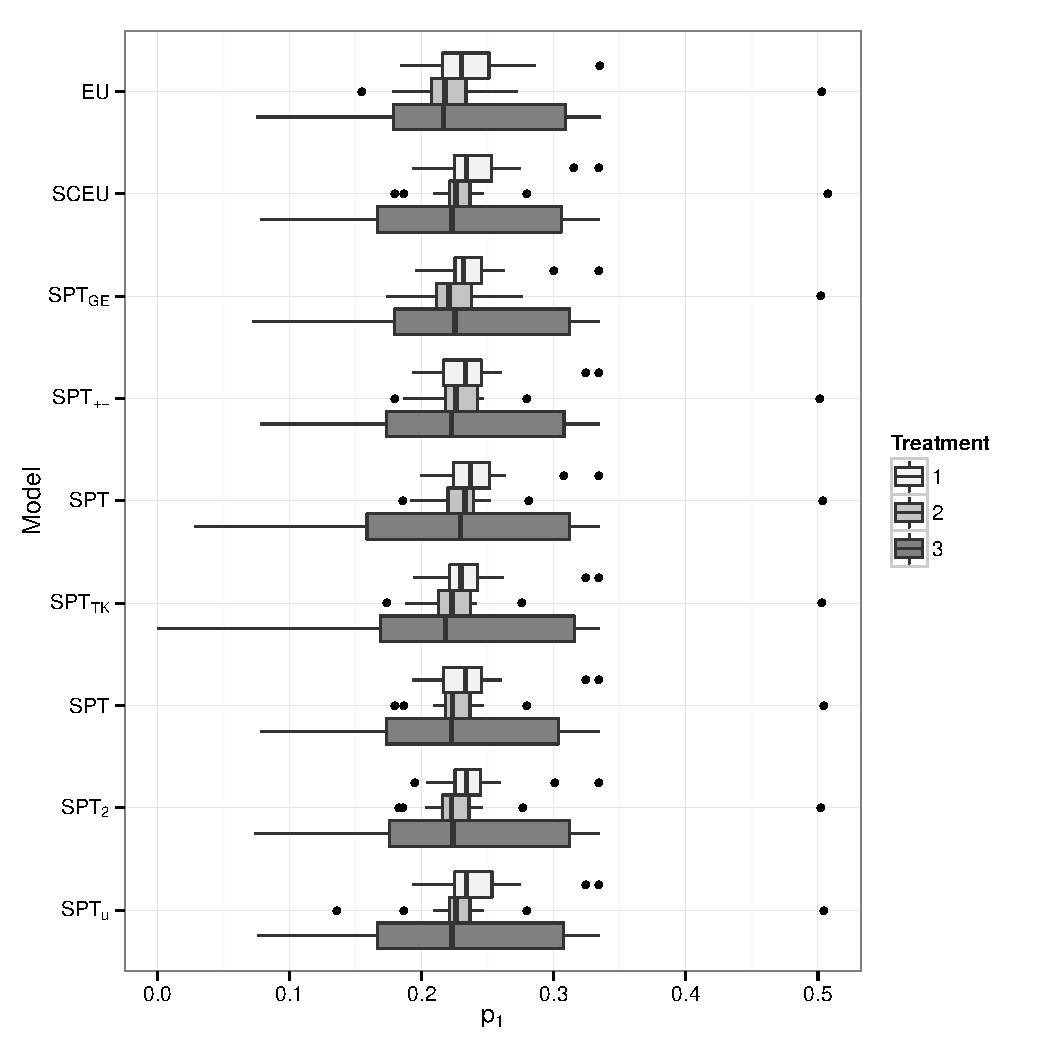
\includegraphics[width=\maxwidth]{figure/p1_boxplot-1} \caption[Individual estimates of the subjective probability of the pink ball (objective probability ]{Individual estimates of the subjective probability of the pink ball (objective probability $0.2$)}\label{fig:p1_boxplot}
\end{figure}




\begin{figure}
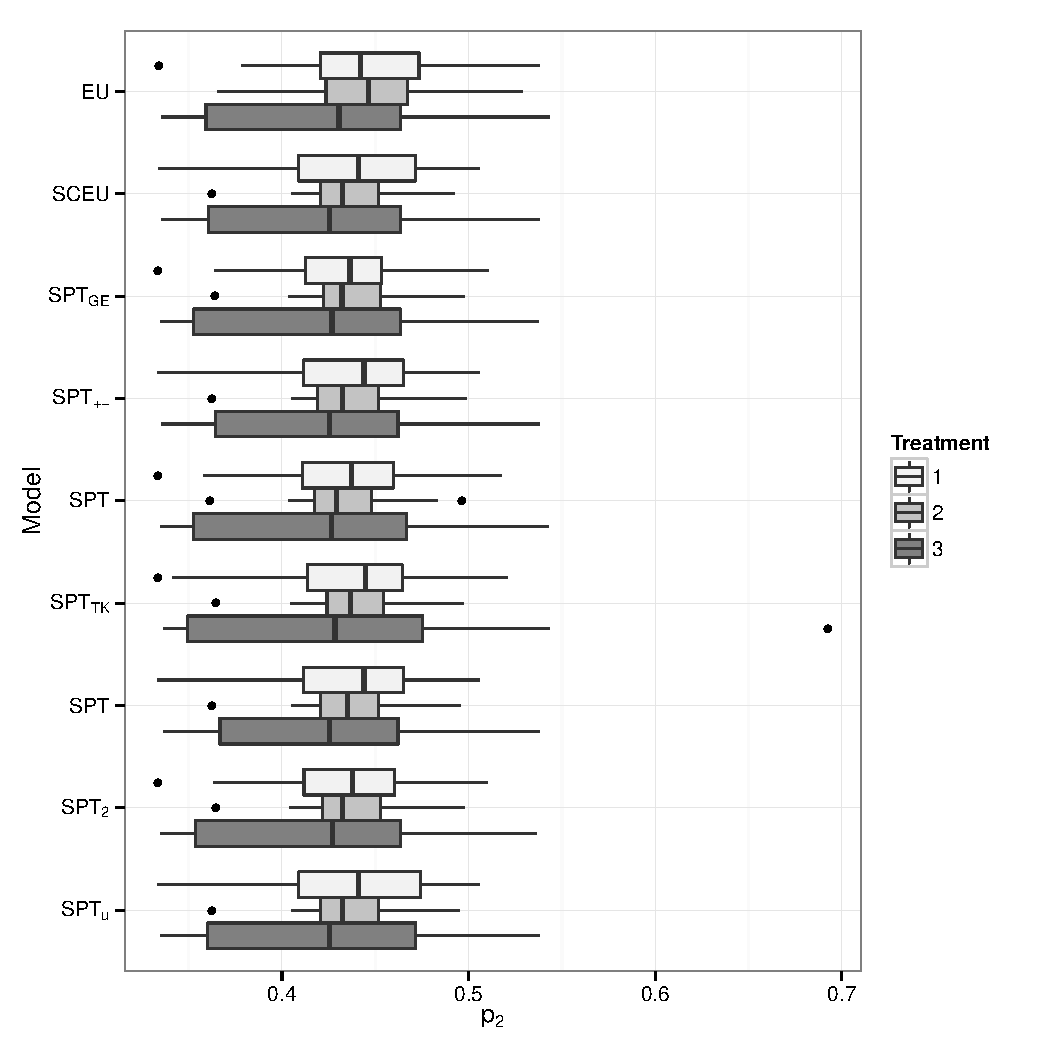
\includegraphics[width=\maxwidth]{figure/p2_boxplot-1} \caption[Individual estimates of the subjective probability of the blue ball (objective probability ]{Individual estimates of the subjective probability of the blue ball (objective probability $0.3$)}\label{fig:p2_boxplot}
\end{figure}



It is also remarkable that the probability weighting parameters (reflecting ambiguity attitudes here) in general suggest more  S-shaped weighting than  inverse S-shaped weighting, deviating from the common findings in the literature (also for ambiguity).  This is similar to HLM's finding that maxmax EU fits very well, and maxmin does worse.  Both these findings suggest that these data contain more optimism than pessimism in event weighting, in deviation from findings in other papers.  HLM give no explanation for this unusual finding.  We have no explanation for it either, and we can only confirm HLM's finding here.

\section{Cross Validation}
\label{sec:cross-validation}

As an additional test of our main hypothesis (that SPT performs best on this given dataset) and to rule out the posibility that our findings are a consequence of the particular fit/test data split, we performed a cross-validation analysis. We randomly split the total of 162 questions in 10 roughly equal batches. For each batch $i\in\{1, \ldots, 10\}$ we estimated the parameters of all the models excluding batch $i$. Then we computed the predicted
 log-likelihood on the test batch $i$. To aggregate the predicted
 log-likelihood across 10 batches, we used medians (Table~\ref{table_ACV1_cros_val_median}) and trimmed(0.1) means (Table~\ref{table_ACV2_cros_val_mean_.1}). The results of this analysis are very similar to those presented in the main text.  This finding confirms that the choice of the test and prediction samples of HLM, followed by us in the main text, are representative.


% latex table generated in R 3.1.1 by xtable 1.7-4 package
% Tue Jun 16 15:28:44 2015
\begin{table}[!htb]
\centering
\begin{tabular}{rllllllllllll}
  \hline
 & SPT & SPT$_{u}$ & SCEU & CEU$_{u}$ & $\alpha$MM & PT & PT$_{u}$ & MnEU & MxEU & EU & CEV & SCEV \\ 
  \hline
SPT$_{u}$ & $22^{\stackrel{\textstyle26\hfill}{\scriptscriptstyle\hfill}}$ & - & - & - & - & - & - & - & - & - & - & - \\ 
  SCEU & $24^{\stackrel{\textstyle24\hfill}{\scriptscriptstyle\hfill}}$ & $25^{\stackrel{\textstyle23\hfill}{\scriptscriptstyle\hfill}}$ & - & - & - & - & - & - & - & - & - & - \\ 
  CEU$_{u}$ & $11^{\stackrel{\textstyle37\hfill}{\scriptscriptstyle***\hfill}}$ & $15^{\stackrel{\textstyle33\hfill}{\scriptscriptstyle***\hfill}}$ & $15^{\stackrel{\textstyle33\hfill}{\scriptscriptstyle***\hfill}}$ & - & - & - & - & - & - & - & - & - \\ 
  $\alpha$MM & $18^{\stackrel{\textstyle30\hfill}{\scriptscriptstyle*\hfill}}$ & $17^{\stackrel{\textstyle31\hfill}{\scriptscriptstyle*\hfill}}$ & $20^{\stackrel{\textstyle28\hfill}{\scriptscriptstyle\hfill}}$ & $27^{\stackrel{\textstyle21\hfill}{\scriptscriptstyle\hfill}}$ & - & - & - & - & - & - & - & - \\ 
  PT & $13^{\stackrel{\textstyle35\hfill}{\scriptscriptstyle***\hfill}}$ & $15^{\stackrel{\textstyle33\hfill}{\scriptscriptstyle***\hfill}}$ & $14^{\stackrel{\textstyle34\hfill}{\scriptscriptstyle***\hfill}}$ & $26^{\stackrel{\textstyle22\hfill}{\scriptscriptstyle\hfill}}$ & $19^{\stackrel{\textstyle29\hfill}{\scriptscriptstyle\hfill}}$ & - & - & - & - & - & - & - \\ 
  PT$_{u}$ & $13^{\stackrel{\textstyle35\hfill}{\scriptscriptstyle***\hfill}}$ & $16^{\stackrel{\textstyle32\hfill}{\scriptscriptstyle***\hfill}}$ & $15^{\stackrel{\textstyle33\hfill}{\scriptscriptstyle***\hfill}}$ & $24^{\stackrel{\textstyle24\hfill}{\scriptscriptstyle\hfill}}$ & $21^{\stackrel{\textstyle27\hfill}{\scriptscriptstyle\hfill}}$ & $24^{\stackrel{\textstyle24\hfill}{\scriptscriptstyle\hfill}}$ & - & - & - & - & - & - \\ 
  MnEU & $16^{\stackrel{\textstyle32\hfill}{\scriptscriptstyle*\hfill}}$ & $18^{\stackrel{\textstyle30\hfill}{\scriptscriptstyle*\hfill}}$ & $18^{\stackrel{\textstyle30\hfill}{\scriptscriptstyle*\hfill}}$ & $26^{\stackrel{\textstyle22\hfill}{\scriptscriptstyle\hfill}}$ & $23^{\stackrel{\textstyle25\hfill}{\scriptscriptstyle\hfill}}$ & $27^{\stackrel{\textstyle21\hfill}{\scriptscriptstyle\hfill}}$ & $27^{\stackrel{\textstyle21\hfill}{\scriptscriptstyle\hfill}}$ & - & - & - & - & - \\ 
  MxEU & $19^{\stackrel{\textstyle29\hfill}{\scriptscriptstyle*\hfill}}$ & $18^{\stackrel{\textstyle30\hfill}{\scriptscriptstyle*\hfill}}$ & $20^{\stackrel{\textstyle28\hfill}{\scriptscriptstyle\hfill}}$ & $27^{\stackrel{\textstyle21\hfill}{\scriptscriptstyle\hfill}}$ & $21^{\stackrel{\textstyle27\hfill}{\scriptscriptstyle\hfill}}$ & $27^{\stackrel{\textstyle21\hfill}{\scriptscriptstyle\hfill}}$ & $25^{\stackrel{\textstyle23\hfill}{\scriptscriptstyle\hfill}}$ & $24^{\stackrel{\textstyle24\hfill}{\scriptscriptstyle\hfill}}$ & - & - & - & - \\ 
  EU & $18^{\stackrel{\textstyle30\hfill}{\scriptscriptstyle*\hfill}}$ & $19^{\stackrel{\textstyle29\hfill}{\scriptscriptstyle\hfill}}$ & $18^{\stackrel{\textstyle30\hfill}{\scriptscriptstyle\hfill}}$ & $26^{\stackrel{\textstyle22\hfill}{\scriptscriptstyle\hfill}}$ & $19^{\stackrel{\textstyle29\hfill}{\scriptscriptstyle\hfill}}$ & $27^{\stackrel{\textstyle21\hfill}{\scriptscriptstyle\hfill}}$ & $26^{\stackrel{\textstyle22\hfill}{\scriptscriptstyle\hfill}}$ & $26^{\stackrel{\textstyle22\hfill}{\scriptscriptstyle\hfill}}$ & $21^{\stackrel{\textstyle27\hfill}{\scriptscriptstyle\hfill}}$ & - & - & - \\ 
  CEV & $5^{\stackrel{\textstyle43\hfill}{\scriptscriptstyle***\hfill}}$ & $5^{\stackrel{\textstyle43\hfill}{\scriptscriptstyle***\hfill}}$ & $5^{\stackrel{\textstyle43\hfill}{\scriptscriptstyle***\hfill}}$ & $12^{\stackrel{\textstyle36\hfill}{\scriptscriptstyle***\hfill}}$ & $10^{\stackrel{\textstyle38\hfill}{\scriptscriptstyle***\hfill}}$ & $13^{\stackrel{\textstyle35\hfill}{\scriptscriptstyle**\hfill}}$ & $13^{\stackrel{\textstyle35\hfill}{\scriptscriptstyle**\hfill}}$ & $10^{\stackrel{\textstyle38\hfill}{\scriptscriptstyle***\hfill}}$ & $10^{\stackrel{\textstyle38\hfill}{\scriptscriptstyle***\hfill}}$ & $9^{\stackrel{\textstyle39\hfill}{\scriptscriptstyle***\hfill}}$ & - & - \\ 
  SCEV & $2^{\stackrel{\textstyle46\hfill}{\scriptscriptstyle***\hfill}}$ & $1^{\stackrel{\textstyle47\hfill}{\scriptscriptstyle***\hfill}}$ & $1^{\stackrel{\textstyle47\hfill}{\scriptscriptstyle***\hfill}}$ & $7^{\stackrel{\textstyle41\hfill}{\scriptscriptstyle***\hfill}}$ & $4^{\stackrel{\textstyle44\hfill}{\scriptscriptstyle***\hfill}}$ & $9^{\stackrel{\textstyle39\hfill}{\scriptscriptstyle***\hfill}}$ & $9^{\stackrel{\textstyle39\hfill}{\scriptscriptstyle***\hfill}}$ & $5^{\stackrel{\textstyle43\hfill}{\scriptscriptstyle***\hfill}}$ & $5^{\stackrel{\textstyle43\hfill}{\scriptscriptstyle***\hfill}}$ & $4^{\stackrel{\textstyle44\hfill}{\scriptscriptstyle***\hfill}}$ & $12^{\stackrel{\textstyle36\hfill}{\scriptscriptstyle***\hfill}}$ & - \\ 
  EV & $2^{\stackrel{\textstyle46\hfill}{\scriptscriptstyle***\hfill}}$ & $2^{\stackrel{\textstyle46\hfill}{\scriptscriptstyle***\hfill}}$ & $2^{\stackrel{\textstyle46\hfill}{\scriptscriptstyle***\hfill}}$ & $9^{\stackrel{\textstyle39\hfill}{\scriptscriptstyle***\hfill}}$ & $4^{\stackrel{\textstyle44\hfill}{\scriptscriptstyle***\hfill}}$ & $9^{\stackrel{\textstyle39\hfill}{\scriptscriptstyle***\hfill}}$ & $11^{\stackrel{\textstyle37\hfill}{\scriptscriptstyle***\hfill}}$ & $4^{\stackrel{\textstyle44\hfill}{\scriptscriptstyle***\hfill}}$ & $4^{\stackrel{\textstyle44\hfill}{\scriptscriptstyle***\hfill}}$ & $2^{\stackrel{\textstyle46\hfill}{\scriptscriptstyle***\hfill}}$ & $12^{\stackrel{\textstyle36\hfill}{\scriptscriptstyle***\hfill}}$ & $24^{\stackrel{\textstyle24\hfill}{\scriptscriptstyle\hfill}}$ \\ 
   \hline
\end{tabular}
\caption{Winner counts with Wilkinson statistics (based on median predicted log-likelihood across 10 batches).} 
\label{table_ACV1_cros_val_median}
\end{table}
% latex table generated in R 3.1.1 by xtable 1.7-4 package
% Tue Jun 16 15:28:44 2015
\begin{table}[!htb]
\centering
\begin{tabular}{rllllllllllll}
  \hline
 & SPT & SPT$_{u}$ & SCEU & CEU$_{u}$ & $\alpha$MM & PT & PT$_{u}$ & MnEU & MxEU & EU & CEV & SCEV \\ 
  \hline
SPT$_{u}$ & $22^{\stackrel{\textstyle26\hfill}{\scriptscriptstyle\hfill}}$ & - & - & - & - & - & - & - & - & - & - & - \\ 
  SCEU & $24^{\stackrel{\textstyle24\hfill}{\scriptscriptstyle\hfill}}$ & $25^{\stackrel{\textstyle23\hfill}{\scriptscriptstyle\hfill}}$ & - & - & - & - & - & - & - & - & - & - \\ 
  CEU$_{u}$ & $11^{\stackrel{\textstyle37\hfill}{\scriptscriptstyle***\hfill}}$ & $15^{\stackrel{\textstyle33\hfill}{\scriptscriptstyle***\hfill}}$ & $15^{\stackrel{\textstyle33\hfill}{\scriptscriptstyle***\hfill}}$ & - & - & - & - & - & - & - & - & - \\ 
  $\alpha$MM & $18^{\stackrel{\textstyle30\hfill}{\scriptscriptstyle*\hfill}}$ & $17^{\stackrel{\textstyle31\hfill}{\scriptscriptstyle*\hfill}}$ & $20^{\stackrel{\textstyle28\hfill}{\scriptscriptstyle\hfill}}$ & $27^{\stackrel{\textstyle21\hfill}{\scriptscriptstyle\hfill}}$ & - & - & - & - & - & - & - & - \\ 
  PT & $13^{\stackrel{\textstyle35\hfill}{\scriptscriptstyle***\hfill}}$ & $15^{\stackrel{\textstyle33\hfill}{\scriptscriptstyle***\hfill}}$ & $14^{\stackrel{\textstyle34\hfill}{\scriptscriptstyle***\hfill}}$ & $26^{\stackrel{\textstyle22\hfill}{\scriptscriptstyle\hfill}}$ & $19^{\stackrel{\textstyle29\hfill}{\scriptscriptstyle\hfill}}$ & - & - & - & - & - & - & - \\ 
  PT$_{u}$ & $13^{\stackrel{\textstyle35\hfill}{\scriptscriptstyle***\hfill}}$ & $16^{\stackrel{\textstyle32\hfill}{\scriptscriptstyle***\hfill}}$ & $15^{\stackrel{\textstyle33\hfill}{\scriptscriptstyle***\hfill}}$ & $24^{\stackrel{\textstyle24\hfill}{\scriptscriptstyle\hfill}}$ & $21^{\stackrel{\textstyle27\hfill}{\scriptscriptstyle\hfill}}$ & $24^{\stackrel{\textstyle24\hfill}{\scriptscriptstyle\hfill}}$ & - & - & - & - & - & - \\ 
  MnEU & $16^{\stackrel{\textstyle32\hfill}{\scriptscriptstyle*\hfill}}$ & $18^{\stackrel{\textstyle30\hfill}{\scriptscriptstyle*\hfill}}$ & $18^{\stackrel{\textstyle30\hfill}{\scriptscriptstyle*\hfill}}$ & $26^{\stackrel{\textstyle22\hfill}{\scriptscriptstyle\hfill}}$ & $23^{\stackrel{\textstyle25\hfill}{\scriptscriptstyle\hfill}}$ & $27^{\stackrel{\textstyle21\hfill}{\scriptscriptstyle\hfill}}$ & $27^{\stackrel{\textstyle21\hfill}{\scriptscriptstyle\hfill}}$ & - & - & - & - & - \\ 
  MxEU & $19^{\stackrel{\textstyle29\hfill}{\scriptscriptstyle*\hfill}}$ & $18^{\stackrel{\textstyle30\hfill}{\scriptscriptstyle*\hfill}}$ & $20^{\stackrel{\textstyle28\hfill}{\scriptscriptstyle\hfill}}$ & $27^{\stackrel{\textstyle21\hfill}{\scriptscriptstyle\hfill}}$ & $21^{\stackrel{\textstyle27\hfill}{\scriptscriptstyle\hfill}}$ & $27^{\stackrel{\textstyle21\hfill}{\scriptscriptstyle\hfill}}$ & $25^{\stackrel{\textstyle23\hfill}{\scriptscriptstyle\hfill}}$ & $24^{\stackrel{\textstyle24\hfill}{\scriptscriptstyle\hfill}}$ & - & - & - & - \\ 
  EU & $18^{\stackrel{\textstyle30\hfill}{\scriptscriptstyle*\hfill}}$ & $19^{\stackrel{\textstyle29\hfill}{\scriptscriptstyle\hfill}}$ & $18^{\stackrel{\textstyle30\hfill}{\scriptscriptstyle\hfill}}$ & $26^{\stackrel{\textstyle22\hfill}{\scriptscriptstyle\hfill}}$ & $19^{\stackrel{\textstyle29\hfill}{\scriptscriptstyle\hfill}}$ & $27^{\stackrel{\textstyle21\hfill}{\scriptscriptstyle\hfill}}$ & $26^{\stackrel{\textstyle22\hfill}{\scriptscriptstyle\hfill}}$ & $26^{\stackrel{\textstyle22\hfill}{\scriptscriptstyle\hfill}}$ & $21^{\stackrel{\textstyle27\hfill}{\scriptscriptstyle\hfill}}$ & - & - & - \\ 
  CEV & $5^{\stackrel{\textstyle43\hfill}{\scriptscriptstyle***\hfill}}$ & $5^{\stackrel{\textstyle43\hfill}{\scriptscriptstyle***\hfill}}$ & $5^{\stackrel{\textstyle43\hfill}{\scriptscriptstyle***\hfill}}$ & $12^{\stackrel{\textstyle36\hfill}{\scriptscriptstyle***\hfill}}$ & $10^{\stackrel{\textstyle38\hfill}{\scriptscriptstyle***\hfill}}$ & $13^{\stackrel{\textstyle35\hfill}{\scriptscriptstyle**\hfill}}$ & $13^{\stackrel{\textstyle35\hfill}{\scriptscriptstyle**\hfill}}$ & $10^{\stackrel{\textstyle38\hfill}{\scriptscriptstyle***\hfill}}$ & $10^{\stackrel{\textstyle38\hfill}{\scriptscriptstyle***\hfill}}$ & $9^{\stackrel{\textstyle39\hfill}{\scriptscriptstyle***\hfill}}$ & - & - \\ 
  SCEV & $2^{\stackrel{\textstyle46\hfill}{\scriptscriptstyle***\hfill}}$ & $1^{\stackrel{\textstyle47\hfill}{\scriptscriptstyle***\hfill}}$ & $1^{\stackrel{\textstyle47\hfill}{\scriptscriptstyle***\hfill}}$ & $7^{\stackrel{\textstyle41\hfill}{\scriptscriptstyle***\hfill}}$ & $4^{\stackrel{\textstyle44\hfill}{\scriptscriptstyle***\hfill}}$ & $9^{\stackrel{\textstyle39\hfill}{\scriptscriptstyle***\hfill}}$ & $9^{\stackrel{\textstyle39\hfill}{\scriptscriptstyle***\hfill}}$ & $5^{\stackrel{\textstyle43\hfill}{\scriptscriptstyle***\hfill}}$ & $5^{\stackrel{\textstyle43\hfill}{\scriptscriptstyle***\hfill}}$ & $4^{\stackrel{\textstyle44\hfill}{\scriptscriptstyle***\hfill}}$ & $12^{\stackrel{\textstyle36\hfill}{\scriptscriptstyle***\hfill}}$ & - \\ 
  EV & $2^{\stackrel{\textstyle46\hfill}{\scriptscriptstyle***\hfill}}$ & $2^{\stackrel{\textstyle46\hfill}{\scriptscriptstyle***\hfill}}$ & $2^{\stackrel{\textstyle46\hfill}{\scriptscriptstyle***\hfill}}$ & $9^{\stackrel{\textstyle39\hfill}{\scriptscriptstyle***\hfill}}$ & $4^{\stackrel{\textstyle44\hfill}{\scriptscriptstyle***\hfill}}$ & $9^{\stackrel{\textstyle39\hfill}{\scriptscriptstyle***\hfill}}$ & $11^{\stackrel{\textstyle37\hfill}{\scriptscriptstyle***\hfill}}$ & $4^{\stackrel{\textstyle44\hfill}{\scriptscriptstyle***\hfill}}$ & $4^{\stackrel{\textstyle44\hfill}{\scriptscriptstyle***\hfill}}$ & $2^{\stackrel{\textstyle46\hfill}{\scriptscriptstyle***\hfill}}$ & $12^{\stackrel{\textstyle36\hfill}{\scriptscriptstyle***\hfill}}$ & $24^{\stackrel{\textstyle24\hfill}{\scriptscriptstyle\hfill}}$ \\ 
   \hline
\end{tabular}
\caption{Winner counts with Wilkinson statistics (based on trimmed (0.01) mean of predicted log-likelihood across 10 batches).} 
\label{table_ACV2_cros_val_mean_.1}
\end{table}


\end{document}



%%% Local Variables: 
%%% TeX-master: t
%%% End: 







9


